% fancytikzposter.tex, version 2.1
% Original template created by Elena Botoeva [botoeva@inf.unibz.it], June 2012
% 
% This file is distributed under the Creative Commons Attribution-NonCommercial 2.0
% Generic (CC BY-NC 2.0) license
% http://creativecommons.org/licenses/by-nc/2.0/ 


\documentclass{a0poster}

\usepackage{fancytikzposter}


%%%%% --------- Change here if you want ---------- %%%%%
%% margin for the geometry package, must be changed before using the geometry package
%% default value is 4cm
\setmargin{2}

%% the space between the blocks
%% default value is 2cm
\setblockspacing{1}

%% the height of the title stripe in block nodes, decrease it to save space
%% default value is 3cm
% \setblocktitleheight{3}

%% the number of columns in the poster, possible values 2,3
%% default value is 2
% \setcolumnnumber{3}

%% the space between two or more groups of authors from different institutions
%% used in \maketitle
% \setinstituteshift{10}

%% which template to use
%% N1 simple, standard look, with a colored background and gray boxes
%% N2 board with nodes
%% N3 another standard look
%% N4 envelope-like look
%% N5 with a wave-like head, original idea taken from
%%%% http://fc09.deviantart.net/fs71/f/2010/322/1/1/scientific_poster_by_nabuy-d333ria.jpg
\usetemplate{2}

%% components of the templates
%% (the maximal possible numbers are mentioned as the parameters)
% \usecolortemplate{4}
% \usebackgroundtemplate{5}
% \usetitletemplate{2}
\useblocknodetemplate{3}
\useplainblocktemplate{4}
\useinnerblocktemplate{1}


%% the height of the head drawing on top 
%% applicable to templates N3, 4 and 5
% \setheaddrawingheight{14}


%% change the basic colors
%\definecolor{myblue}{HTML}{008888} 
%\setfirstcolor{myblue}% default 116699
%\setsecondcolor{gray!80!}% default CCCCCC
%\setthirdcolor{red!80!black}% default 991111

\definecolor{colblue}{RGB}{1, 33, 105}

%% change the more specific colors
\setbackgrounddarkcolor{teal!5!white}
\setbackgroundlightcolor{teal!5!white}
% \settitletextcolor{textcolor}
% \settitlefillcolor{white}
% \settitledrawcolor{colortwo}
% \setblocktextcolor{textcolor}
% \setblockfillcolor{white}
\setblocktitletextcolor{colorone}
\setblocktitlefillcolor{colortwo} %the color of the border
% \setplainblocktextcolor{textcolor}
% \setplainblockfillcolor{colorthree!40!}
% \setplainblocktitletextcolor{textcolor}
% \setplainblocktitlefillcolor{colorthree!60!}
% \setinnerblocktextcolor{textcolor}
% \setinnerblockfillcolor{white}
% \setinnerblocktitletextcolor{white}
% \setinnerblocktitlefillcolor{colorthree}




%%% size of the document and the margins
%% A0
% \usepackage[margin=\margin cm, paperwidth=118.9cm, paperheight=84.1cm]{geometry} 
% \usepackage[margin=\margin cm, paperwidth=84.1cm, paperheight=118.9cm]{geometry}
%% B1
% \usepackage[margin=\margin cm, paperwidth=70cm, paperheight=100cm]{geometry}

\usepackage[
    margin=\margin cm,
    paperwidth=24in,
    paperheight=36in,
]{geometry}


% \usepackage{fontspec}

%% changing the fonts
% \usepackage{cmbright}
\usepackage[default]{cantarell}
% \usepackage{courier}
%\usepackage{avant}
% \usepackage[math]{iwona}
% \usepackage{lmodern}
% \usepackage[math]{kurier}
% \usepackage[T1]{fontenc}


%% add your packages here
\usepackage{graphicx}
\usepackage{hyperref}
\usepackage{enumitem}
\usepackage[scr]{rsfso}
\usepackage{bm}

\newcommand{\N}{\mathbb{N}}
\newcommand{\Z}{\mathbb{Z}}
\newcommand{\Q}{\mathbb{Q}}
\newcommand{\R}{\mathbb{R}}
\newcommand{\C}{\mathbb{C}}

\newcommand{\iid}{\overset{iid}{\sim}}
\renewcommand{\Pr}{\mathbb{P}}
\newcommand{\E}{\mathbb{E}}





\title{%
    \vspace{0.5cm}
    \huge
    Image Segmentation with Spatial Priors
}
\author{%
    \large Satvik Saha\\
    \normalsize Department of Statistics, Columbia University
}


\begin{document}

\ClearShipoutPicture
\AddToShipoutPicture{\BackgroundPicture}

\noindent % to have the picture right in the center
\begin{tikzpicture}
    \initializesizeandshifts
    % \setxshift{15}
    % \setyshift{2}

    \ifthenelse{\equal{\template}{1}}{ 
        \titleblock{47}{1}
    }{
        \titleblock{47}{1.5}
    }

    \blocknode{Segmentation with Mixture Models}{
        Let $x_\ell \in \mathbb{R}^d$ be the color of a pixel at location $\ell
        \in \mathcal{L}$.
        A $K$-component mixture model generates an image $\bm{x}$ via
        \begin{align*}
            \bm{\theta} &\sim p(\bm{\theta}), \\
            \bm{\beta} &\sim p(\bm{\beta}), \\
            \bm{z} \mid \bm{\beta}
                &\sim p(\bm{z} \mid \bm{\beta}), \\
            x_\ell \mid \bm{\theta}, z_\ell = k
                &\sim p(x_\ell \mid \theta_k, z_\ell = k), \quad\ell \in \mathcal{L}.
        \end{align*}
        Segmentation involves inferring the distribution of labels $\bm{z}\mid \bm{x}$.
    }

    \blocknode{Na\"ive Mixture Models}{
        Simply choosing $z_\ell \mid \bm{\beta} \iid p(\;\cdot \mid
        \bm{\beta})$ ignores spatial information, and uses only the observed
        distribution of color $\bm{x}$; shuffling the locations of all pixels
        would produce the same labels!
        This can produce rough, grainy segments with `islands'.

        \begin{tikzfigure}[%
            A na\"ive mixture model only sees the distribution of $x_\ell$.
        ]
        \begin{tabular}{c@{\hskip 1em}c}
            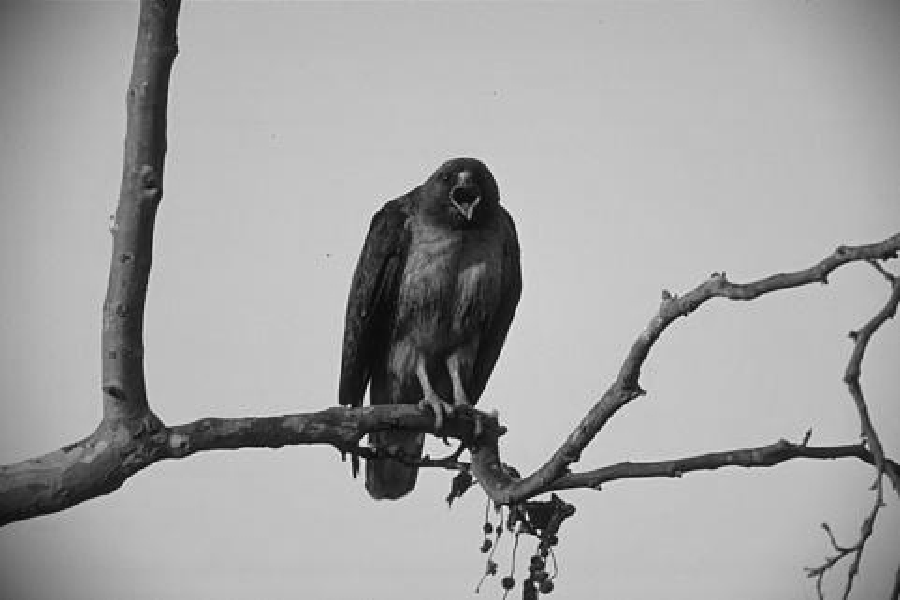
\includegraphics[width=0.48\textwidth]{42049_grey} &
            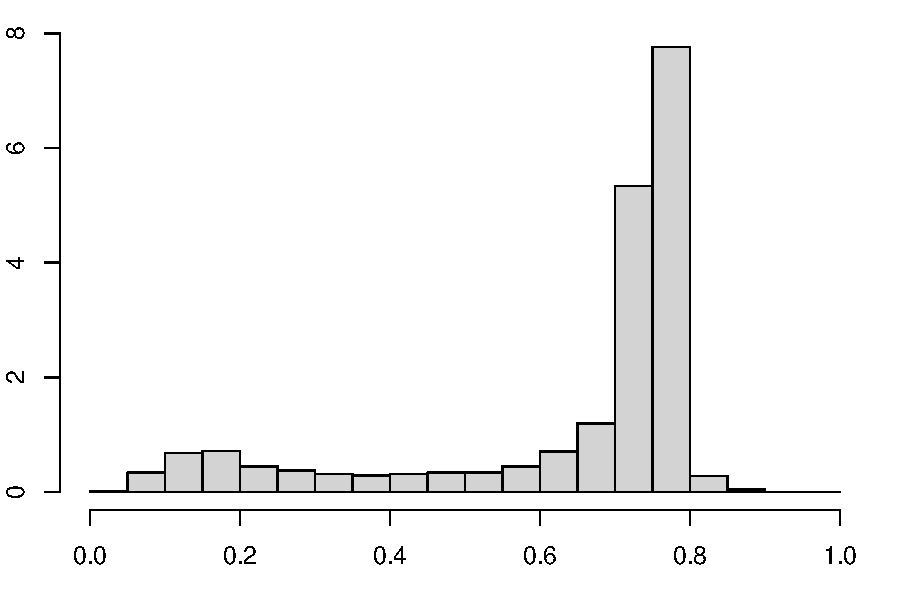
\includegraphics[width=0.48\textwidth]{42049_grey_hist} \\
            Grayscale image & Distribution of $x_\ell$
        \end{tabular}
        \end{tikzfigure}

        We will focus on one particular aspect of spatial information, and use
        the following heuristic: \emph{neighboring pixels often belong to the
        same segment}.
    }

    \blocknode{Potts-Markov Spatial Priors}{
        Given some description $\mathcal{G}(\mathcal{L}, \mathcal{E})$ of pixel
        neighborhoods, consider \[
            p(\bm{z}\mid \bm{\beta})
                = \frac{1}{Z(\bm{\beta})}\,\exp\left(\sum_{\ell \sim \ell'}\sum_{k = 1}^K \beta_k \bm{1}(z_\ell = z_{\ell'} = k)\right)
                = \frac{\exp(\bm{\beta}^\top \bm{T}(\bm{z}))}{Z(\bm{\beta})}.
        \]
        This rewards assigning neighboring pixels the same label, producing
        `smoother' segments.

        % \begin{tikzfigure}%[Draws from $p(\bm{z} \mid \bm{\beta})$]
        % \begin{tabular}{c@{\hskip 1em}c@{\hskip 1em}c}
        %     
\includegraphics[width=0.26\textwidth]{potts_beta_0} &
        %     
\includegraphics[width=0.26\textwidth]{potts_beta_1} &
        %     
\includegraphics[width=0.26\textwidth]{potts_beta_custom} \\
        %     $\bm\beta = \bm0$ &
        %     $\bm\beta = \bm1$ &
        %     $\bm\beta = (1, 1.5, 1.5)^\top$
        % \end{tabular}
        % \end{tikzfigure}

        \vspace{1em}
        \begin{tikzfigure}[%
            Draws from $p(\bm{z} \mid \bm{\beta})$, using Gibbs sampling.
        ]
        \begin{tabular}{c@{\hskip 2em}c@{\hskip 2em}c}
            
\includegraphics[width=0.32\textwidth]{potts_beta_0} &
            
\includegraphics[width=0.32\textwidth]{potts_beta_1} \\
            $\bm\beta = \bm0$ & $\bm\beta = \bm1$ \\\\
            
\includegraphics[width=0.32\textwidth]{potts_beta_10} &
            
\includegraphics[width=0.32\textwidth]{potts_beta_custom} \\
            $\bm\beta = \bm{10}$ & $\bm\beta = (1, 1.5, 1.5)^\top$
        \end{tabular}
        \end{tikzfigure}
    }

    %%%%%%%%%%%%% NEW COLUMN %%%%%%%%%%%%%%% 
    \startsecondcolumn 


    \blocknode{Gaussian-GIW-Potts Mixture}{
        Using the Potts-Markov spatial prior, we further choose 
        \begin{align*}
            \beta_k
                &\iid \text{Gamma}(a_\beta, b_\beta), \\
            \Sigma_k
                &\iid \text{Inv-Wishart}(\Sigma_k; \Sigma_0, \nu_0), \\
            \mu_k \mid \Sigma_k
                &\sim \text{Normal}(m_0, \kappa_0^{-1}\Sigma_k), \\
            x_\ell \mid \mu_k, \Sigma_k, z_\ell = k
                &\sim \text{Normal}(\mu_k, \Sigma_k).
        \end{align*}
        \vspace{-2em}
        \begin{tikzfigure}[%
            Image segmentation, with $K = 5$.
        ]
        \begin{tabular}{c@{\hskip 1em}c}
            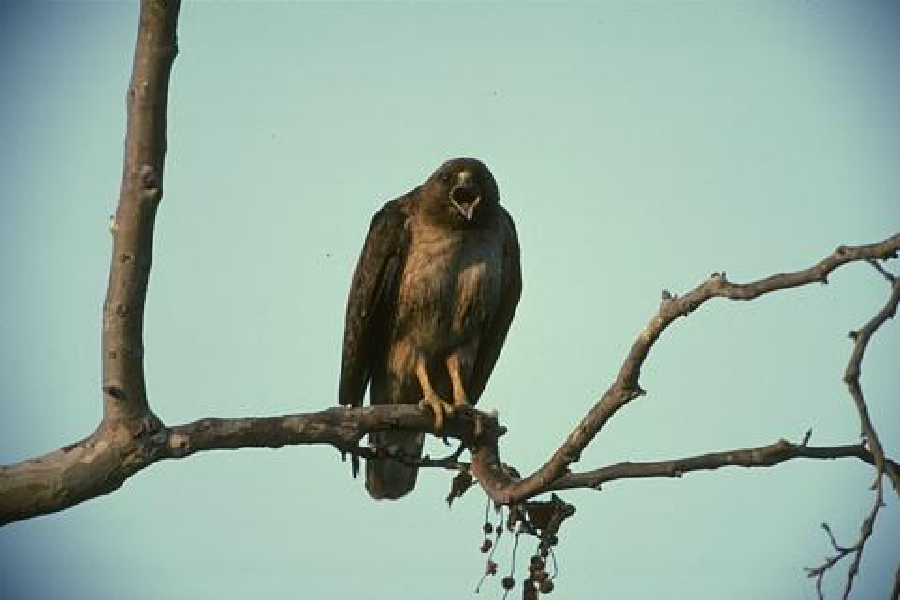
\includegraphics[width=0.48\textwidth]{42049_orig} &
            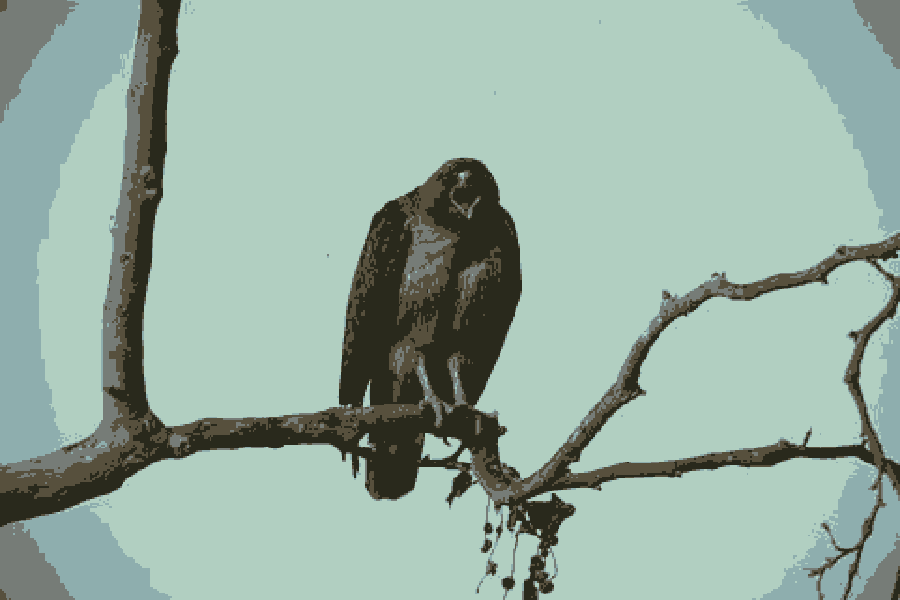
\includegraphics[width=0.48\textwidth]{42049_K5_seg_kmeans} \\
            Original & K-Means \\\\
            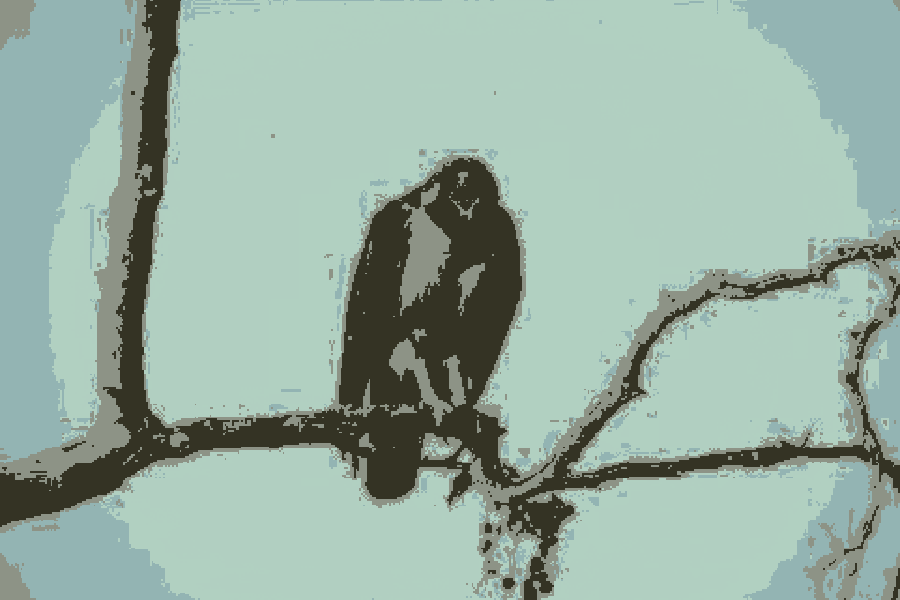
\includegraphics[width=0.48\textwidth]{42049_K5_seg_gmm} &
            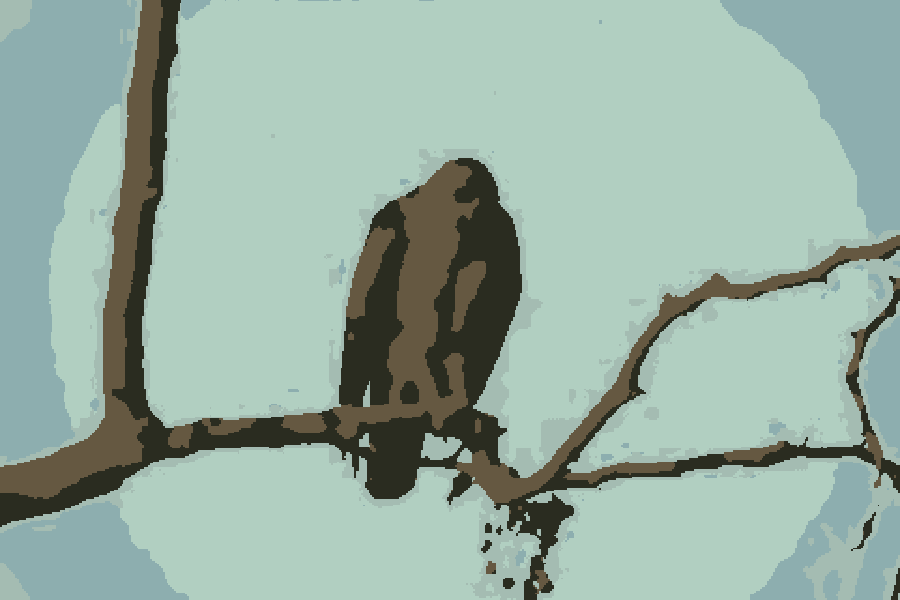
\includegraphics[width=0.48\textwidth]{42049_K5_seg_fixed} \\
            GMM & GGIWP-MM, $\bm\beta = \bm{1}$ \\\\
            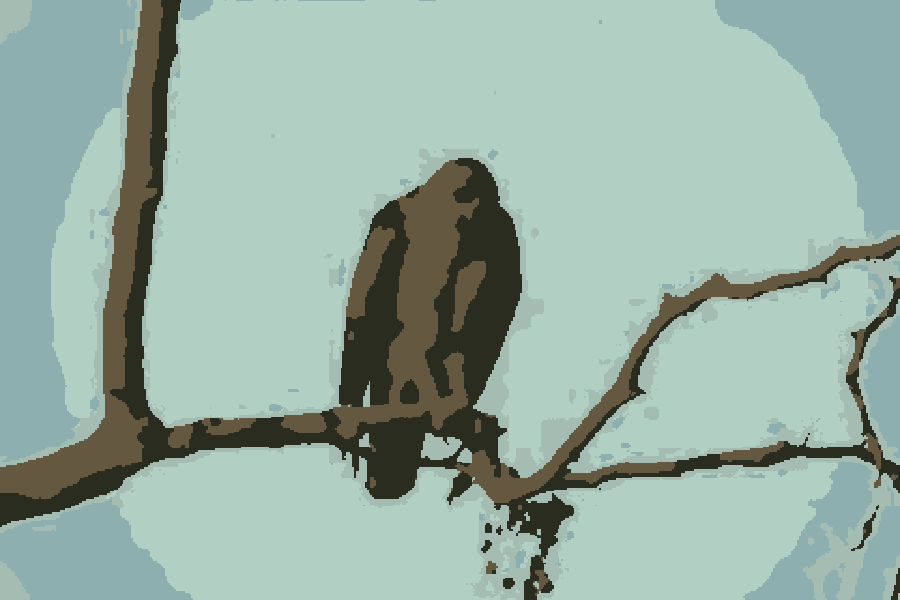
\includegraphics[width=0.48\textwidth]{42049_K5_seg} &
            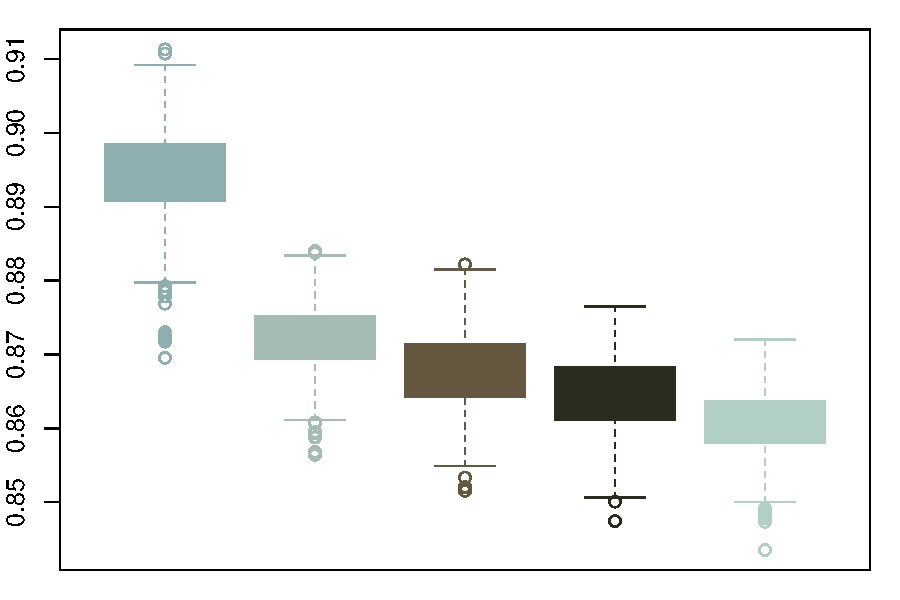
\includegraphics[width=0.48\textwidth]{42049_K5_beta} \\
            GGIWP-MM & Posterior summary of $\bm{\beta}$
        \end{tabular}
        \end{tikzfigure}
        \vspace{1em}

        The posterior distribution of $\bm\beta$ gives information about the
        smoothness of each segment.
    }


    \blocknode{Auxiliary Variable MCMC}{
        In this model, the joint likelihood itself is intractable.
        Specifically, it is difficult to draw from the full-conditional \[
            p(\bm{\beta} \mid \bm{z})
                \propto \frac{p(\bm{\beta})}{Z(\bm{\beta})}\,\exp\left(\bm{\beta}^\top \bm{T}(\bm{z})\right).
        \] For instance, a Metropolis-Hastings acceptance ratio depends on the
        intractable term $Z(\bm{\beta}^*)/Z(\bm{\beta})$. \\

        To circumvent this, we use an auxiliary variable \emph{exchange
        algorithm} (\textcolor{colblue}{M\o ller et al., 2004}):
        \begin{enumerate}[leftmargin=2em]
            \item Propose $\bm{\beta}^* \sim q(\bm{\beta}^*; \bm{\beta})$.
            \item Draw auxiliary $\bm{z}^* \sim p(\bm{z}^* \mid \bm{\beta}^*)$.
            \item Accept $\bm{\beta}^*$ with probability \[
                \frac{
                    q(\bm{\beta}; \bm{\beta}^*)\,
                    p(\bm{\beta}^*)
                }{
                    q(\bm{\beta}^*; \bm{\beta})\,
                    p(\bm{\beta})
                }\cdot \frac{
                    p(\bm{z} \mid \bm{\beta}^*)
                }{
                    p(\bm{z} \mid \bm{\beta})
                }\cdot \frac{
                    p(\bm{z}^*\mid \bm{\beta})
                }{
                    p(\bm{z}^* \mid \bm{\beta}^*)
                }.
            \]
        \end{enumerate}

        This is fairly expensive (Gibbs within Metropolis-Hastings within
        Gibbs), but yields the correct posterior as its stationary
        distribution!
    }


\end{tikzpicture}
\end{document}
